\documentclass[12pt]{article}
\usepackage[margin=1.5cm]{geometry}
\usepackage{parskip}
\usepackage{amsmath}
\usepackage{amssymb}
\usepackage{amsfonts}
\usepackage{enumitem}
\usepackage{graphicx}
\usepackage{stmaryrd}
\graphicspath{ {./images/} }


\begin{document}
\begin{enumerate}[label=(\alph*)]

  \item
    For pairwise sequence alignment, we can use a dynamic programming algorithm to compute the optimal pairwise alignment by building a 2D edit graph, and computing an alignment score for every node, and then backtracking from the bottom-right cell to compute the alignment itself.

    Since computing each cell takes $O(1)$ time, and our edit graph is $n \times n$ (assuming the two sequences are of equal length), the complexity for the algorithm is $O(n^2)$.

    Scaling this up for multiple alignment means that, say if we were aligning 3 sequences, then instead of building a 2D edit graph, we have to build a 3D edit graph. For $m$ sequences, we build an $m$-dimensional edit graph. Furthermore, the dynamic programming function we evaluate to compute the alignment score is no longer constant time, since instead of having a constant number of options to choose, the number of options we have scales with $m$, so we have $O(2^m)$ options. Then, since we have $n^m$ cells, our total runtime is $O(c^{2m})$

    This is simply too slow, so for multiple alignments we opt to use an algorithm like CLUSTAL, which can instead take $O(n^2)$ time (or higher, depending on which algorithm is used to build the guide tree, but likely not more than $O(n^3)$).

    \item
      When we are aligning DNA sequences, we want our alignment scores to be representative of the underlying biological truth, i.e. how biologically different are the DNA sequences. When we see gaps during our alignment, in biology it is likely that these occur from a single genetic event, as opposed to many independent genetic events, so we want to punish gap openings more than gap extension, which leads us to an affine gap penalty (as opposed to a usual constant gap penalty).

      This can be implemented by duplicating our edit graph 3 times, and `jumping' to different levels depending on whether we open or close a gap (and in what direction).

      \item
        Not relevant.

        \item
The UPGMA algorithm is an algorithm to compute a phylogenetic tree from a distance matrix between the species, where the distances are usually calculated with similarity scores of their DNA sequences.


The algorithm works by progressively clustering nodes into a parent, until we reach a single node.

It takes as input a distance matrix, and returns as output a rooted tree, where each leaf is one of the original species.

We begin with every node in its own cluster. Then, we iterate the following steps until we reach a single cluster:

Merge the two clusters that are closest to each other into a single node. Set the branch lengths to be half of the distance between the two clusters.

Remove the two clusters from the distance matrix, them and replace them with a merged cluster, where the distance between the merged cluster and the other clusters is given by the average distance between each pair of nodes across the clusters.

Consider the following example:

Suppose we have the following distance matrix:

\begin{tabular}{c|c|c|c|c}
  &a&b&c&d\\
  \hline
  a&0&2&10&11\\
  \hline
  b& &0&8&9\\
  \hline
  c& & &0&4\\
  \hline
  d& & & &0
\end{tabular}

UPGMA gives us the following tree:

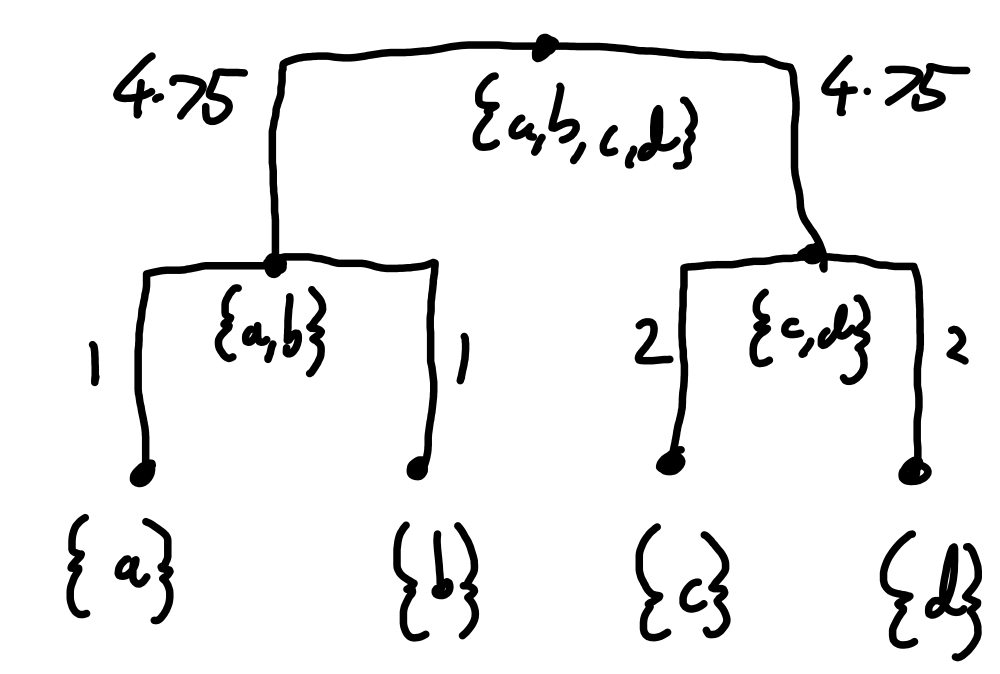
\includegraphics[scale=0.3]{upgma}

And the following intermediate distance matrices:


\begin{tabular}{c|c|c|c}
  &a,b&c&d\\
  \hline
  a,b&0&9&10\\
  \hline
  c& &0&4\\
  \hline
  d& & &0
\end{tabular}

\begin{tabular}{c|c|c}
  &a,b&c,d\\
  \hline
  a,b&0&9.5\\
  \hline
  c,d& &0\\
\end{tabular}

A trivial implementation of this algorithm has time complexity $O(n^3)$ and $O(n^2)$ space complexity, although an implementation exists that has $O(n^2)$ time complexity and $O(n^2)$ space complexity.

The UPGMA algorithm ensures that the resulting tree is ultrametric.

The UPGMA algorithm can produce a tree for any distance matrix, unlike the additive phylogeny algorithm for example, but does not always produce the `best' trees. For example, if a matrix is additive, then we do not necessarily produce its corresponding simple tree, but an algorithm like neighbour-joining will.

\item
  The ultrametric property of a tree (like those produced by UPGMA) means that the distance from the root to any leaf is the same. Since we assume the species at the leaf nodes to be in existence at the same time, this means that ultrametric trees have that the distances represent time, assuming that we have a molecular clock (where the quantity of genetic mutations we have is proportional to time).


        
    \end{enumerate}
\end{document}
